% Block diagram / data flow for miniproj.v (IERG2820 mini project)
% Standalone TikZ figure. Compile with pdflatex.
\documentclass[tikz,border=7pt]{standalone}
\usepackage[T1]{fontenc}
\usepackage{lmodern}
\usepackage{amsmath,amssymb}
\usetikzlibrary{arrows.meta,positioning,calc,fit,backgrounds}

\definecolor{cdata}{RGB}{25,25,28}
\definecolor{cctrl}{RGB}{20,85,160}
\definecolor{ctick}{RGB}{200,105,0}
\definecolor{cflag}{RGB}{105,105,110}
\definecolor{cdpfill}{RGB}{235,243,252}
\definecolor{ccalc}{RGB}{228,239,251}
\definecolor{calu}{RGB}{233,244,235}
\definecolor{csync}{RGB}{255,244,226}
\definecolor{cctrlfill}{RGB}{235,241,250}
\definecolor{cdisp}{RGB}{243,236,250}
\definecolor{cout}{RGB}{240,240,240}

\newcommand{\hdr}[1]{\textbf{\small #1}}

\begin{document}
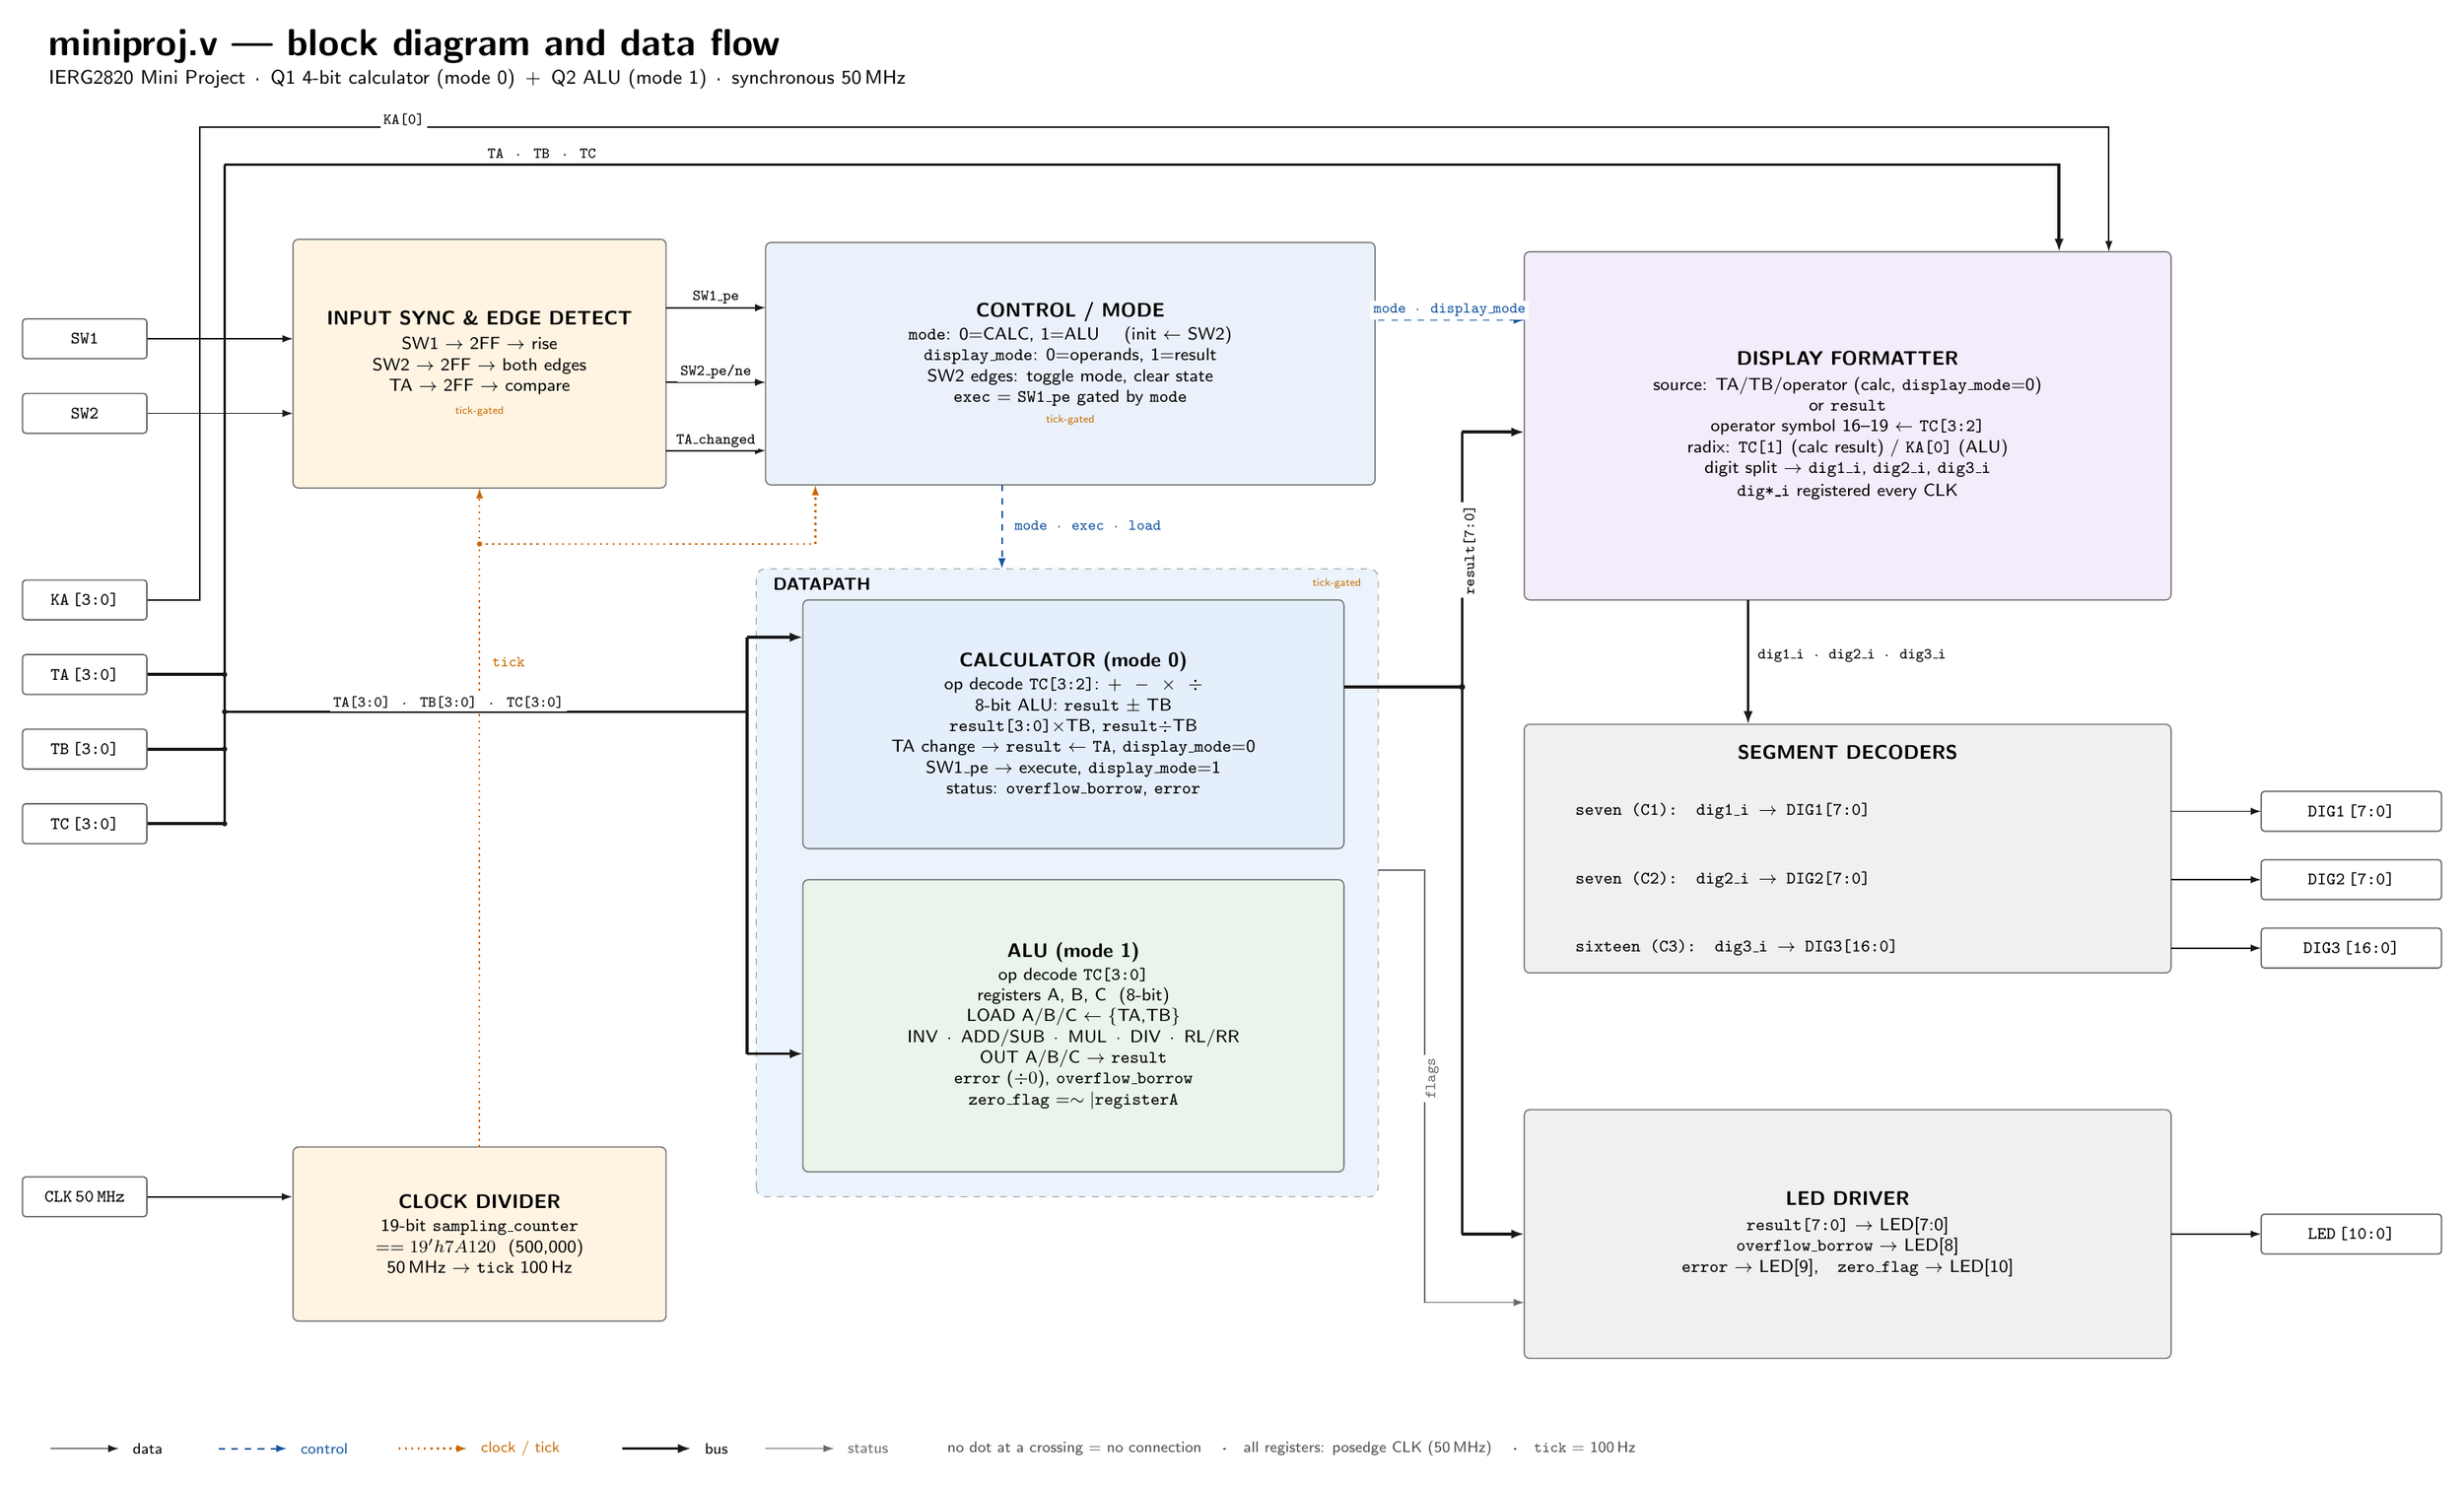
\begin{tikzpicture}[
  x=1cm, y=1cm,
  font=\sffamily\footnotesize,
  >=Latex,
  blk/.style={draw=black!55, line width=0.55pt, rounded corners=2.5pt,
              align=center, inner sep=3.5pt},
  port/.style={draw=black!60, line width=0.6pt, rounded corners=1.5pt,
               fill=white, minimum width=2.0cm, minimum height=0.64cm,
               align=center, font=\ttfamily\footnotesize, inner sep=2pt},
  opins/.style={draw=black!60, line width=0.6pt, rounded corners=1.5pt,
               fill=white, minimum width=2.9cm, minimum height=0.64cm,
               align=center, font=\ttfamily\footnotesize, inner sep=2pt},
  data/.style={draw=cdata, line width=0.65pt,
               -{Latex[length=1.7mm,width=1.2mm]}},
  datan/.style={draw=cdata, line width=0.65pt},
  bus/.style={draw=cdata, line width=1.3pt,
              -{Latex[length=2.1mm,width=1.5mm]}},
  busn/.style={draw=cdata, line width=1.3pt},
  ctrl/.style={draw=cctrl, line width=0.7pt, dashed,
               -{Latex[length=1.7mm,width=1.2mm]}},
  ctrln/.style={draw=cctrl, line width=0.7pt, dashed},
  tickl/.style={draw=ctick, line width=0.9pt, dotted,
                -{Latex[length=1.7mm,width=1.2mm]}},
  tickn/.style={draw=ctick, line width=0.9pt, dotted},
  flag/.style={draw=cflag, line width=0.65pt,
               -{Latex[length=1.7mm,width=1.2mm]}},
  lbl/.style={font=\ttfamily\scriptsize, inner sep=1.4pt, fill=white},
  clbl/.style={font=\sffamily\scriptsize, text=cctrl, inner sep=1.4pt, fill=white},
  tlbl/.style={font=\sffamily\scriptsize, text=ctick, inner sep=1.4pt, fill=white},
  flbl/.style={font=\ttfamily\scriptsize, text=cflag, inner sep=1.4pt, fill=white},
  dot/.style={fill=cdata, circle, inner sep=0pt, minimum size=2.4pt},
]

% ------------------------------------------------------------------ title
\node[anchor=west, align=left] at (0.55,22.9) {%
  {\sffamily\LARGE\bfseries miniproj.v --- block diagram and data flow}\\[2pt]
  {\sffamily\small IERG2820 Mini Project \,\textperiodcentered\, Q1 4-bit calculator (mode 0) \,+\, Q2 ALU (mode 1) \,\textperiodcentered\, synchronous 50\,MHz}};

% ------------------------------------------------------------------ inputs
\node[port] (SW1) at (1.25,18.4) {SW1};
\node[port] (SW2) at (1.25,17.2) {SW2};
\node[port] (KA)  at (1.25,14.2) {KA\,[3:0]};
\node[port] (TA)  at (1.25,13.0) {TA\,[3:0]};
\node[port] (TB)  at (1.25,11.8) {TB\,[3:0]};
\node[port] (TC)  at (1.25,10.6) {TC\,[3:0]};
\node[port] (CLK) at (1.25,4.6)  {CLK\,50\,MHz};

% ------------------------------------------------------------------ sync + divider
\node[blk, fill=csync, minimum width=6.0cm, minimum height=4.0cm]
  (sync) at (7.6,18.0) {%
  \hdr{INPUT SYNC \& EDGE DETECT}\\[2pt]
  SW1 $\to$ 2FF $\to$ rise\\
  SW2 $\to$ 2FF $\to$ both edges\\
  TA $\to$ 2FF $\to$ compare\\[1pt]
  {\color{ctick}\sffamily\tiny tick-gated}};

\node[blk, fill=csync, minimum width=6.0cm, minimum height=2.8cm]
  (counter) at (7.6,4.0) {%
  \hdr{CLOCK DIVIDER}\\[1pt]
  19-bit \texttt{sampling\_counter}\\
  $==19'h7A120$ \ (500{,}000)\\
  50\,MHz $\to$ \texttt{tick} 100\,Hz};

% ------------------------------------------------------------------ control
\node[blk, fill=cctrlfill, minimum width=9.8cm, minimum height=3.9cm]
  (control) at (17.1,18.0) {%
  \hdr{CONTROL / MODE}\\[1pt]
  \texttt{mode}: 0=CALC, 1=ALU \quad (init $\leftarrow$ SW2)\\
  \texttt{display\_mode}: 0=operands, 1=result\\
  SW2 edges: toggle mode, clear state\\
  \texttt{exec} = \texttt{SW1\_pe} gated by \texttt{mode}\\
  {\color{ctick}\sffamily\tiny tick-gated}};

% ------------------------------------------------------------------ datapath
\begin{scope}[on background layer]
  \draw[draw=black!40, dashed, rounded corners=4pt, fill=cdpfill]
    (12.05,4.6) rectangle (22.05,14.7);
\end{scope}
\node[anchor=west, font=\sffamily\footnotesize\bfseries] at (12.2,14.46) {DATAPATH};
\node[anchor=east, font=\sffamily\tiny, text=ctick] at (21.9,14.46) {tick-gated};

\node[blk, fill=ccalc, minimum width=8.7cm, minimum height=4.0cm]
  (calc) at (17.15,12.2) {%
  \hdr{CALCULATOR (mode 0)}\\[1pt]
  op decode \texttt{TC[3:2]}: $+$ \ $-$ \ $\times$ \ $\div$\\
  8-bit ALU: \texttt{result} $\pm$ TB\\
  \texttt{result[3:0]}$\times$TB, \texttt{result}$\div$TB\\
  TA change $\to$ \texttt{result} $\leftarrow$ \texttt{TA}, \texttt{display\_mode}=0\\
  SW1\_pe $\to$ execute, \texttt{display\_mode}=1\\
  status: \texttt{overflow\_borrow}, \texttt{error}};

\node[blk, fill=calu, minimum width=8.7cm, minimum height=4.7cm]
  (alu) at (17.15,7.35) {%
  \hdr{ALU (mode 1)}\\[1pt]
  op decode \texttt{TC[3:0]}\\
  registers A, B, C \ (8-bit)\\
  LOAD A/B/C $\leftarrow$ \{TA,TB\}\\
  INV \,\textperiodcentered\, ADD/SUB \,\textperiodcentered\, MUL \,\textperiodcentered\, DIV \,\textperiodcentered\, RL/RR\\
  OUT A/B/C $\to$ \texttt{result}\\
  \texttt{error} ($\div0$), \texttt{overflow\_borrow}\\
  \texttt{zero\_flag} $= \sim|$\texttt{registerA}};

% ------------------------------------------------------------------ display / decoders / LEDs
\node[blk, fill=cdisp, minimum width=10.4cm, minimum height=5.6cm]
  (display) at (29.6,17.0) {%
  \hdr{DISPLAY FORMATTER}\\[2pt]
  source: TA/TB/operator (calc, \texttt{display\_mode}=0)\\
  or \texttt{result}\\
  operator symbol 16--19 $\leftarrow$ \texttt{TC[3:2]}\\
  radix: \texttt{TC[1]} (calc result) / \texttt{KA[0]} (ALU)\\
  digit split $\to$ \texttt{dig1\_i}, \texttt{dig2\_i}, \texttt{dig3\_i}\\[1pt]
  \texttt{dig*\_i} registered every CLK};

% segment decoders: background + explicitly placed rows (aligned with pins)
\node[blk, fill=cout, minimum width=10.4cm, minimum height=4.0cm]
  (dec) at (29.6,10.2) {};
\node[font=\sffamily\small\bfseries] at (29.6,11.75) {SEGMENT DECODERS};
\node[anchor=west, font=\ttfamily\footnotesize] at (25.1,10.8)
  {\texttt{seven} (C1): \texttt{dig1\_i} $\to$ DIG1[7:0]};
\node[anchor=west, font=\ttfamily\footnotesize] at (25.1,9.7)
  {\texttt{seven} (C2): \texttt{dig2\_i} $\to$ DIG2[7:0]};
\node[anchor=west, font=\ttfamily\footnotesize] at (25.1,8.6)
  {\texttt{sixteen} (C3): \texttt{dig3\_i} $\to$ DIG3[16:0]};

\node[blk, fill=cout, minimum width=10.4cm, minimum height=4.0cm]
  (leddrv) at (29.6,4.0) {%
  \hdr{LED DRIVER}\\[2pt]
  \texttt{result[7:0]} $\to$ LED[7:0]\\
  \texttt{overflow\_borrow} $\to$ LED[8]\\
  \texttt{error} $\to$ LED[9],\quad \texttt{zero\_flag} $\to$ LED[10]};

% ------------------------------------------------------------------ output pins
\node[opins] (DIG1) at (37.7,10.8) {DIG1\,[7:0]};
\node[opins] (DIG2) at (37.7,9.7)  {DIG2\,[7:0]};
\node[opins] (DIG3) at (37.7,8.6)  {DIG3\,[16:0]};
\node[opins] (LED)   at (37.7,4.0)  {LED\,[10:0]};

% ------------------------------------------------------------------ clock / tick
\draw[data] (CLK.east) -- (counter.west |- 0,4.6);
\draw[tickl]
  (7.6,5.4) -- (7.6,16.0);
\node[tlbl, anchor=west] at (7.75,13.2) {\texttt{tick}};
% tick branch to control
\draw[tickn]
  (7.6,15.1) -- (13.0,15.1) -- (13.0,15.9);
\draw[tickl] (13.0,15.9) -- (13.0,16.05);
\fill[ctick] (7.6,15.1) circle (1.2pt);

% ------------------------------------------------------------------ switches -> sync
\draw[data] (SW1.east) -- (4.6,18.4);
\draw[data] (SW2.east) -- (4.6,17.2);

% ------------------------------------------------------------------ sync -> control
\draw[data] (10.6,18.9) -- (12.2,18.9);
\draw[data] (10.6,17.7) -- (12.2,17.7);
\draw[data] (10.6,16.6) -- (12.2,16.6);
\node[lbl, above] at (11.4,18.9) {\texttt{SW1\_pe}};
\node[lbl, above] at (11.4,17.7) {\texttt{SW2\_pe/ne}};
\node[lbl, above] at (11.4,16.6) {\texttt{TA\_changed}};

% ------------------------------------------------------------------ operand bus
% bus trunk TA/TB/TC
\draw[busn] (TA.east) -- (3.5,13.0);
\draw[busn] (TB.east) -- (3.5,11.8);
\draw[busn] (TC.east) -- (3.5,10.6);
\draw[busn] (3.5,10.6) -- (3.5,21.2);
\fill[dot] (3.5,13.0) circle (1.2pt);
\fill[dot] (3.5,11.8) circle (1.2pt);
\fill[dot] (3.5,10.6) circle (1.2pt);
% bus to display
\draw[bus] (3.5,21.2) -- (33.0,21.2) -- (33.0,19.8);
% bus tap to datapath
\draw[busn] (3.5,12.4) -- (11.9,12.4);
\fill[dot] (3.5,12.4) circle (1.2pt);
\draw[busn] (11.9,12.4) -- (11.9,13.6);
\draw[bus]  (11.9,13.6) -- (12.8,13.6);
\draw[busn] (11.9,12.4) -- (11.9,6.9);
\draw[bus]  (11.9,6.9) -- (12.8,6.9);
\node[lbl] at (7.1,12.55) {\texttt{TA[3:0]} \,\textperiodcentered\, \texttt{TB[3:0]} \,\textperiodcentered\, \texttt{TC[3:0]}};
\node[lbl] at (8.6,21.38) {\texttt{TA} \,\textperiodcentered\, \texttt{TB} \,\textperiodcentered\, \texttt{TC}};

% KA line to display
\draw[data]
  (KA.east) -- (3.1,14.2) -- (3.1,21.8) -- (33.8,21.8) -- (33.8,19.8);
\node[lbl, anchor=west] at (6.0,21.92) {\texttt{KA[0]}};

% ------------------------------------------------------------------ control -> datapath / display
\draw[ctrl] (16.0,16.05) -- (16.0,14.7);
\node[clbl, anchor=west] at (16.15,15.4) {\texttt{mode \textperiodcentered\ exec \textperiodcentered\ load}};
\draw[ctrl] (22.05,18.7) -- (24.4,18.7);
\node[clbl, above] at (23.2,18.7) {\texttt{mode \textperiodcentered\ display\_mode}};

% ------------------------------------------------------------------ result + flags
\draw[busn] (21.5,12.8) -- (23.4,12.8);
\fill[dot] (23.4,12.8) circle (1.4pt);
% result to display
\draw[busn] (23.4,12.8) -- (23.4,16.9);
\draw[bus]  (23.4,16.9) -- (24.4,16.9);
% result to LED driver
\draw[busn] (23.4,12.8) -- (23.4,4.0);
\draw[bus]  (23.4,4.0) -- (24.4,4.0);
\node[lbl, rotate=90] at (23.52,15.0) {\texttt{result[7:0]}};
% flags
\draw[flag] (22.05,9.85) -- (22.8,9.85) -- (22.8,2.9) -- (24.4,2.9);
\node[flbl, rotate=90] at (22.92,6.5) {\texttt{flags}};

% ------------------------------------------------------------------ display -> decoders
\draw[bus] (28.0,14.2) -- (28.0,12.2);
\node[lbl, anchor=west] at (28.1,13.3) {\texttt{dig1\_i \textperiodcentered\ dig2\_i \textperiodcentered\ dig3\_i}};

% ------------------------------------------------------------------ decoders / LED -> pins
\draw[data] (34.8,10.8) -- (36.25,10.8);
\draw[data] (34.8,9.7)  -- (36.25,9.7);
\draw[data] (34.8,8.6)  -- (36.25,8.6);
\draw[data] (34.8,4.0)  -- (36.25,4.0);

% ------------------------------------------------------------------ legend
\draw[data] (0.7,0.55) -- (1.8,0.55);
\node[anchor=west, font=\sffamily\scriptsize] at (1.9,0.55) {data};
\draw[ctrl] (3.4,0.55) -- (4.5,0.55);
\node[anchor=west, font=\sffamily\scriptsize, text=cctrl] at (4.6,0.55) {control};
\draw[tickl] (6.3,0.55) -- (7.4,0.55);
\node[anchor=west, font=\sffamily\scriptsize, text=ctick] at (7.5,0.55) {clock / tick};
\draw[bus] (9.9,0.55) -- (11.0,0.55);
\node[anchor=west, font=\sffamily\scriptsize] at (11.1,0.55) {bus};
\draw[flag] (12.2,0.55) -- (13.3,0.55);
\node[anchor=west, font=\sffamily\scriptsize, text=cflag] at (13.4,0.55) {status};
\node[anchor=west, font=\sffamily\scriptsize, text=black!70] at (15.0,0.55)
  {no dot at a crossing = no connection \quad\textperiodcentered\quad all registers: posedge CLK (50\,MHz) \quad\textperiodcentered\quad \texttt{tick} = 100\,Hz};

\end{tikzpicture}
\end{document}
